\chapter{Implementation}

This chapter introduces some interesting implementation details and techniques, focusing mainly on the frontend but also mentioning the backend, including the spaced repetition algorithm.

\section{Frontend implementation}

This section presents the completed frontend application, illustrated with pictures, and then describes the solutions used during the implementation, highlighting the exciting features.

\subsection{The frontend application and screenshots}

TODO

\subsection{Project structure}

The project follows a flat folder structure hierarchy inspired by \texttt{The Go Standard Project Layout}\footnote{https://github.com/golang-standards/project-layout}. Figure \ref{fig:frontend-project-structure} shows this folder structure visually.

\begin{figure}[H]
    \centering
    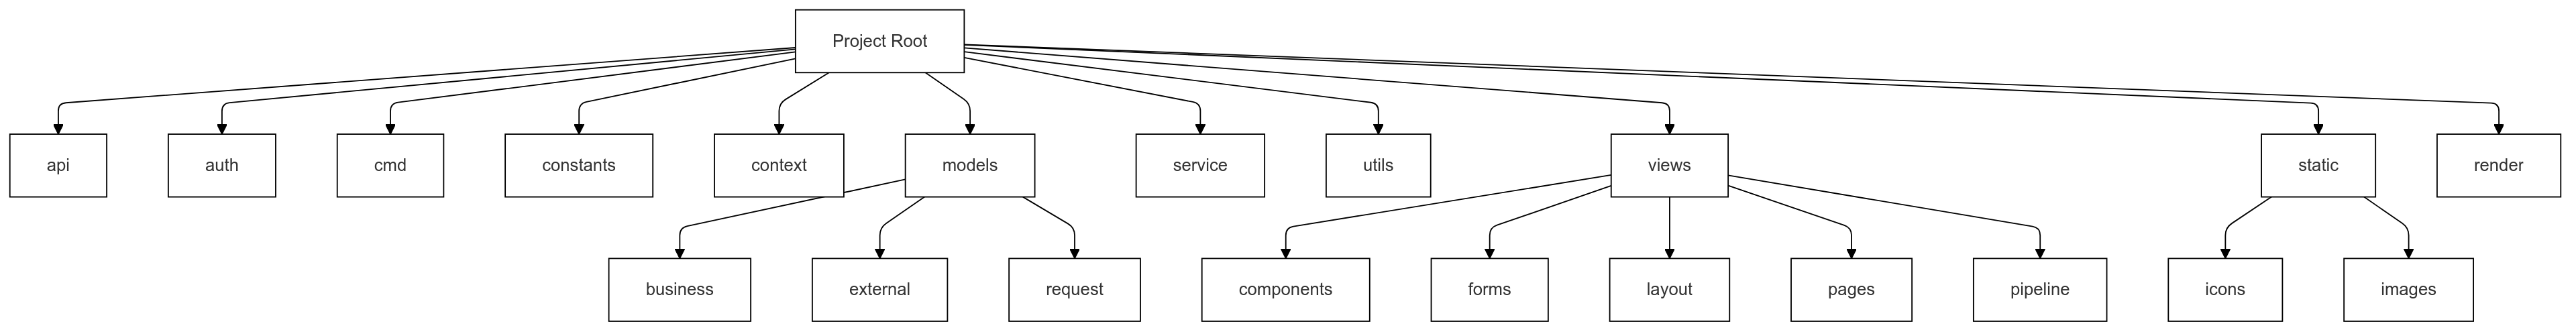
\includegraphics[width=0.8\textwidth, keepaspectratio]{figures/frontend-project-structure.png}
    \caption{Frontend project structure}
    \label{fig:frontend-project-structure}
\end{figure}

\textbf{api}: The \texttt{api} folder contains the endpoint handlers related to the pages and HTMX interactions.

\textbf{auth}: The \texttt{auth} folder contains the endpoint handlers related to the authentication function of the platform.

\textbf{cmd}: The folder \texttt{cmd} is a Go-specific folder containing the main functions. It is a common way to define the entry point of an application in \texttt{cmd/main.go}.

\textbf{constants}: The \texttt{constants} folder contains run-time constants; they wrap the provided environment variables and make them globally available for the application.

\textbf{context}: The \texttt{context} folder contains the custom context of the application. This context includes user information like a session ID and username.

\textbf{models}: The \texttt{models} folder contains Go representations of the data models in different layers and provides mappings between them. There are three layers of data: business, external, and request, which are separated into subfolders.

\textbf{service}: The \texttt{service} folder contains the ApiService, a proxy service providing access to the backend via function calls. This service is accessible through the custom context because the server calls usually require attaching the session ID to the request, and this service can do it automatically.

\textbf{utils}: The \texttt{utils} folder contains utils functions like generating gradient background from UUIDs and finding elements in lists.

\textbf{view}: The \texttt{view} folder contains the templ components and the generated Go code generated from them. They are also separated into subfolders based on their usage: \texttt{components}, \texttt{forms}, \texttt{layout}, \texttt{pages}, and \texttt{pipeline}.

\textbf{static}: The \texttt{static} folder is a regular webserver folder containing static resources for the application, such as scripts, images, and icons.

\textbf{render}: The \texttt{render} folder contains the configuration of the templ renderer and the render pipeline.

\subsection{Data models}

The application operates with three layers of data models. Each has a specific use case and can be mapped into other layer equivalents with mapping functions. These layers are the following: \texttt{business} used for doing the business logic, \texttt{external} used as Data Transfer Objects (DTO), and \texttt{request} used as communicating with the user. Listing \ref{lst:mapping-example} shows an example for mapping a quiz result object from \texttt{external} to \texttt{business} layer.

\begin{lstlisting}[caption=Mapping from external to business,label=lst:mapping-example]
func (result *QuizResult) MapToBusiness() (*business.QuizResult, error) {
    answerScores := make([]business.AnswerScore, 0, len(result.AnswerScores))
    for _, score := range result.AnswerScores {
        answerScore, err := score.MapToBusiness()
        if err != nil {
            return nil, err
        }
        answerScores = append(answerScores, *answerScore)
    }

    return &business.QuizResult{
        ID:           result.ID,
        SessionID:    result.SessionID,
        MaxScore:     result.MaxScore,
        Score:        result.Score,
        AnswerScores: answerScores,
    }, nil
}
\end{lstlisting}

The business layer objects are usually mappings from DTOs, with minor changes for effortless rendering. The DTOs are Go structs with \texttt{struct tags} used for parsing JSON objects. They are mostly the same as used on the backend. The request layer objects are similar to DTOs, but their \texttt{struct tags} help to map form data sent by the client instead of JSON sent by the server.

\subsection{Authentication}

The authentication on the client side is an extension of the server-side version. The user sends the session cookie to the frontend, and the frontend server saves it in the execution context and uses it to fetch data from the backend. A custom context is created from the Echo context on each request by extending it with user-related information and instantiating an ApiService instance. The ApiService automatically attaches the session cookie to the requests before sending them to the backend. Listing~\ref{lst:session-middleware} shows the code of the custom session middleware.

\begin{lstlisting}[caption=Session middleware code,label=lst:session-middleware]
func SessionMiddleware(next echo.HandlerFunc) echo.HandlerFunc {
	return func(c echo.Context) error {
		cc := &AppContext{
			Context: c,
		}

		sessionCookie, err := c.Cookie("session")
		if err != nil {
			return next(cc)
		}

		cc.ApiService = service.NewApiService(sessionCookie)
		session, err := cc.ApiService.GetSession()
		if err != nil {
			return next(cc)
		}

		cc.Session = session
		cc.Set("cc", cc)
		return next(cc)
	}
}
\end{lstlisting}

The custom context creation and session checking are built on the Echo framework middleware feature. I defined a middleware that extends the Echo context and another that checks the extended context to contain the session information. The session creator middleware is placed before every request because it only tries extending the context, but the other one is placed before the execution of the authentication-required endpoint to ensure the user is authenticated. It works like the Angular web framework's Auth guard \footnote{https://angular.dev/api/router/CanActivate} feature. Listing \ref{lst:session-require-middleware} shows the middleware code that ensures the authentication.

\begin{lstlisting}[caption=Session checking middleware code,label=lst:session-require-middleware]
func RequireSessionMiddleware(next echo.HandlerFunc) echo.HandlerFunc {
	return func(c echo.Context) error {
		cc, ok := c.(*AppContext)
		if !ok || cc.Session == nil {
			return c.Redirect(http.StatusFound, "/login")
		}
		return next(c)
	}
}
\end{lstlisting}

\subsection{Rendering pipeline}

I designed a pipeline-like structure for rendering the components to make them easier to manage and use. The pipeline has three stages: two primary and one optional. These stages have different responsibilities and use cases, but they were a good addition to creating a well-organized render structure. The first stage determines the request type, the second renders the desired component(s), and the final extends the rendered component when necessary. The following figure~\ref{fig:rendering-pipeline} shows the whole rendering process.

\begin{figure}[H]
	\centering
	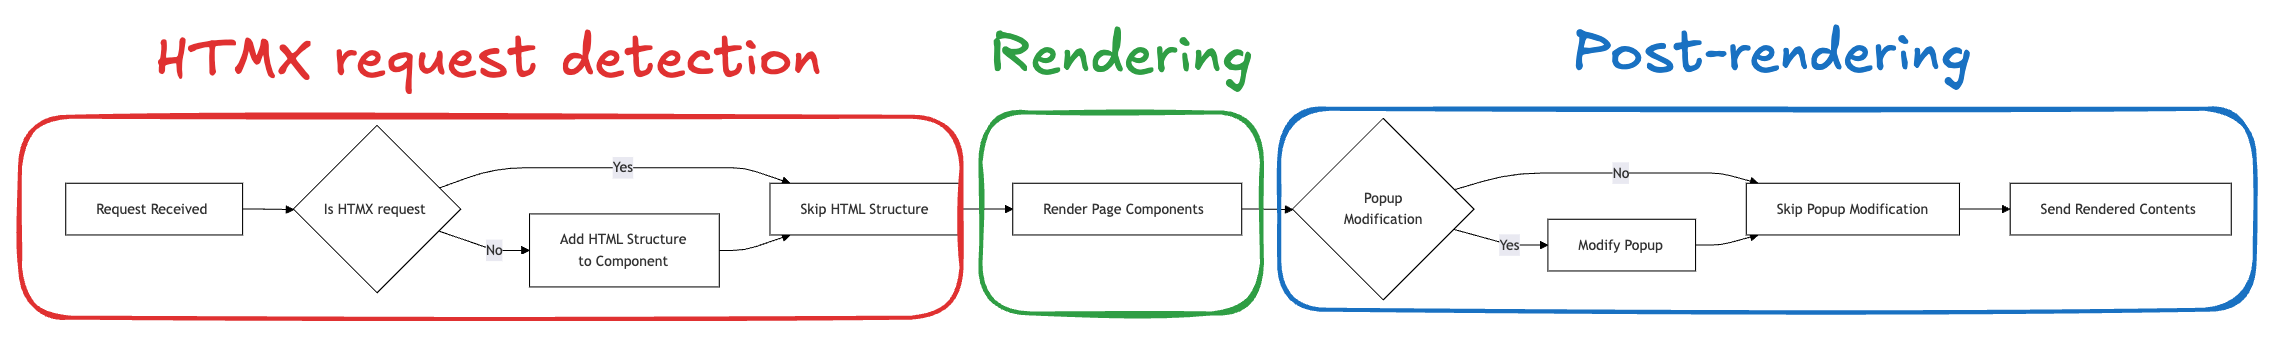
\includegraphics[width=0.8\textwidth, keepaspectratio]{figures/rendering-pipeline.png}
	\caption{Rendering pipeline}
	\label{fig:rendering-pipeline}
\end{figure}

The main problem was rendering the pages in a unified way for different needs. When a user navigates between pages, the frontend server should only render the page and the modified sidebar and let HTMX insert them into the DOM tree. However, when a user accesses a page directly with the URL, the server has to render a base HTML layout containing the scripts and styles in addition to the page and the sidebar—the pipeline's first stage checks whether the incoming request is a standard AJAX or an HTMX-boosted one.

The central stage of the pipeline is responsible for rendering the pages and components. It doesn't have to know whether a rendered element works as it is or is placed into a structure. This stage also allows additional components to be added, but it has to be done manually based on the use case. A common use case is using the HTMX OOB requests to update different parts of an application.

The final stage is responsible for automatically making post-render modifications. Currently, the only use case for this feature in the application is closing popups on navigation. It is made to be extendable, such as keeping a popup open, and can be set, but it has yet to be used.

\subsection{Form handling}

The HTMX requests contain information in HTTP forms. I used an interesting technique \footnote{https://www.youtube.com/watch?v=bQirFmhS3iw} for rendering and validating these forms in the application. The main idea is adding two parameters to the form components; the first is Go struct representing the values filled by the user, and the second is storing error messages. When a user submits a form, the frontend parses the values into the struct and validates them. If any error occurs or a value is inappropriate, the frontend server attaches error messages with keys to the error map and renders the component using the values and the messages. The following listing~\ref{lst:form-handling} shows the login form component's code and how the values and the error messages are set.

\begin{lstlisting}[caption=Login form,label=lst:form-handling]
templ LoginForm(errors map[string]string) {
	<form
		hx-post="/login"
		hx-swap="outerHTML"
		class="flex flex-col gap-y-4 p-6 w-[500px]"
	>
		<span class="text-center text-3xl font-bold">Login</span>
		@components.EMailInput(components.EMailInputProps{
			Error: errors["email"],
		})
		@components.TextInput(components.TextInputProps{
			Name:        "password",
			Label:       "Password",
			Placeholder: "Password",
			Type:        "password",
			Error:       errors["password"],
		})
		@components.Button(components.ButtonProps{
			Text: "Submit",
			Type: "submit",
		})
		@components.LinkButton("Sign up", "/signup", components.ButtonColorWhite)
		if errors["other"] != "" {
			<span class="w-full py-4 text-red-500 text-nowrap">{ errors["other"] }</span>
		}
	</form>
}
\end{lstlisting}

\subsection{Backend integration}

The frontend server makes HTTP requests to the backend endpoints using the ApiService from the context. ApiService is a proxy class that abstracts HTTP requests into function calls. It offers a unified and automated way to communicate with the backend. The session middleware constantly creates one instance for the current context containing the session information. The service's responsibility is to attach the session cookie to each request, and it manages by offering a common request sending and parsing function. This function takes the URL, HTTP method name, request, and response objects as parameters, creates a request, attaches the session cookie to the HTTP header, and processes the request. Listing \ref{lst:api-service} shows the code of this util function.

\begin{lstlisting}[caption=ApiService code,label=lst:api-service]
func (a *ApiService) getResponse(method, path string, requestBody any, responseBody interface{}) error {
	data, err := json.Marshal(requestBody)
	if err != nil {
		return err
	}

	req, err := http.NewRequest(method, constants.BACKEND_URL+path, bytes.NewBuffer(data))
	if err != nil {
		return err
	}

	if a.sessionCookie != nil {
		req.AddCookie(a.sessionCookie)
	}

	resp, err := a.client.Do(req)
	if err != nil {
		return err
	}
	defer resp.Body.Close()

	if resp.StatusCode >= 400 {
		bodyBytes, err := io.ReadAll(resp.Body)
		if err != nil {
			return err
		}

		var result map[string]string
		err = json.Unmarshal(bodyBytes, &result)
		if err != nil {
			return err
		}

		return errors.New("error message: " + result["message"])
	}

	err = json.NewDecoder(resp.Body).Decode(&responseBody)
	if err != nil {
		return err
	}

	return nil
}
\end{lstlisting}